\section{Results}
\label{sec:results}
We report endpoint-level contrasts and keep repeated executions inside each endpoint mean. The results are organized by what each added control changes about the scientific verdict rather than by a universal ``skills help'' narrative.

\subsection{The original-agent anchor overturns a two-arm gain}
\label{sec:falsepositive}
On DeepSeek C3-R cutoff, T succeeds on 100\% of endpoint-repeat observations and the complexity-matched target-blind stress helper G on 72\%. A conventional T-versus-G comparison therefore reports +28 points. N is also 100\%, however, so T--N=0 and the cell is \emph{no repair}. At endpoint means, T--G has 4 wins/1 tie/0 losses, whereas T--N has 0 wins/5 ties/0 losses, so the verdict reversal does not depend on treating repeats as independent tasks. A zero-call audit further confirms equal helper invocation and no detectable condition-position association; T prompts are 18.85 input tokens shorter on average. The point is not that G is a universally fair generic assistant, but that T-versus-stress-helper evidence can look convincingly positive while the original agent was never repaired.

\begin{figure}[t]
\centering
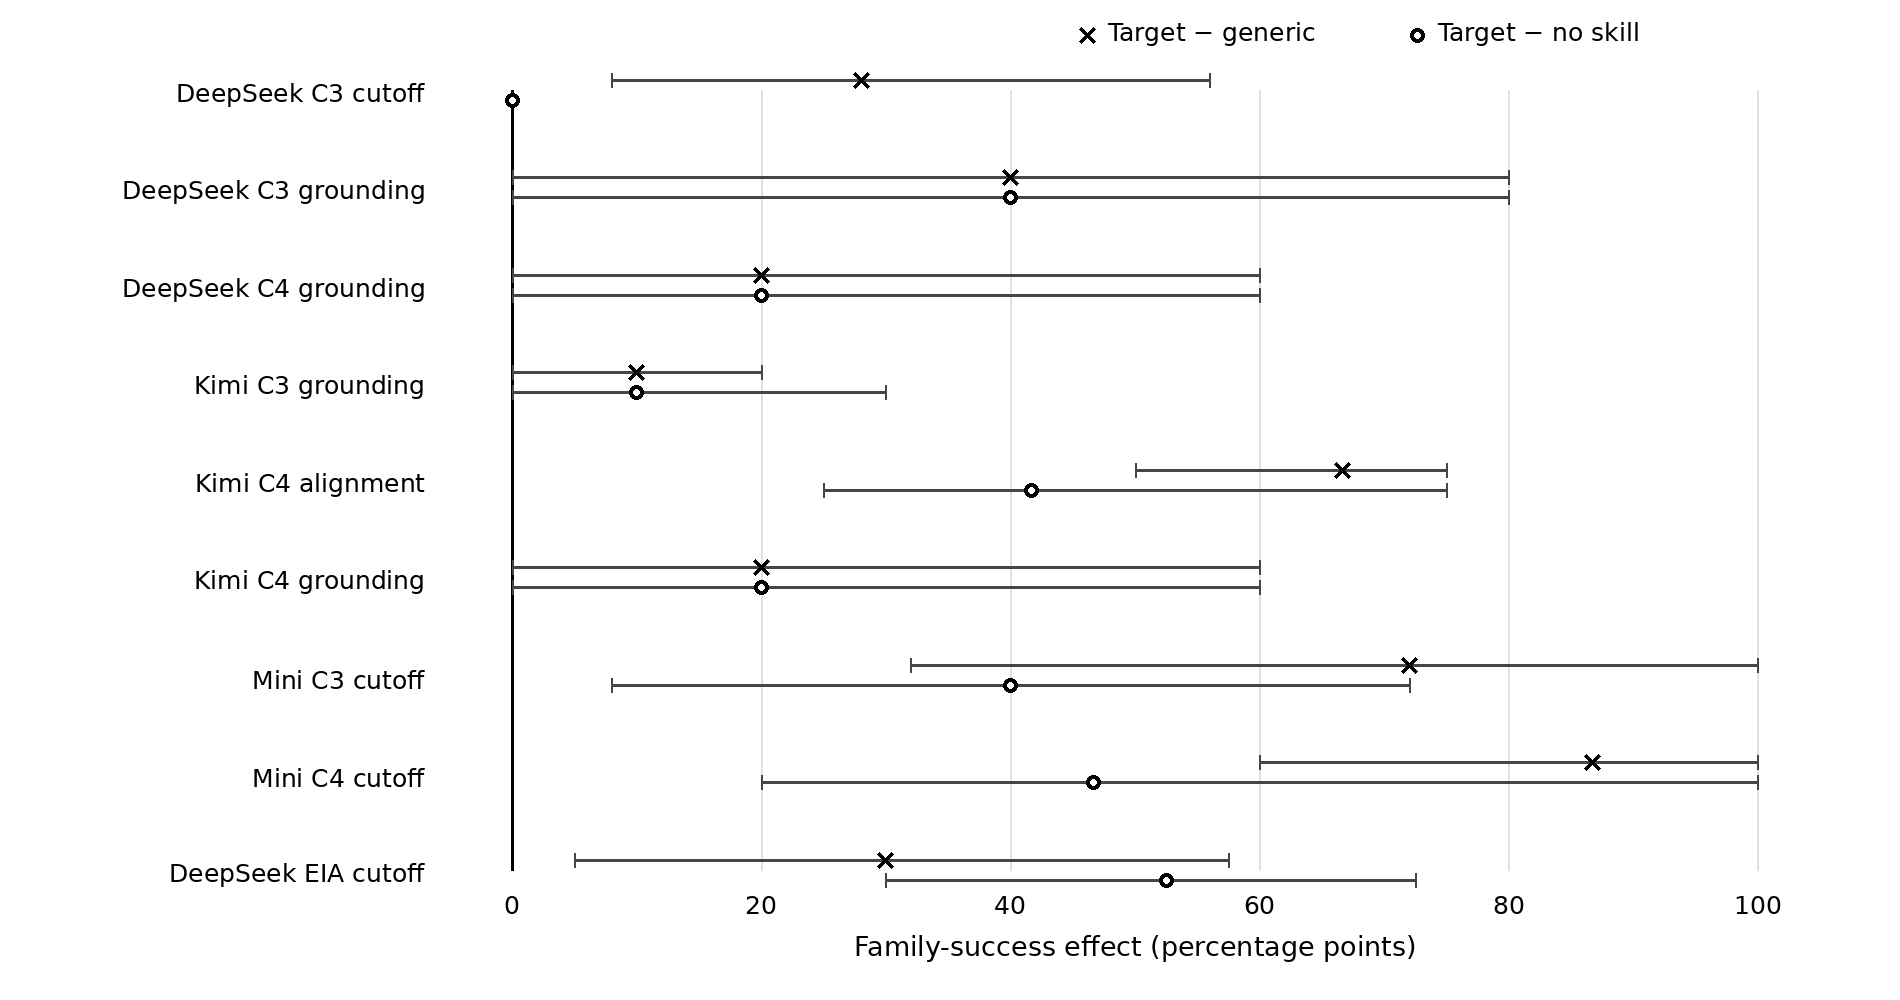
\includegraphics[width=0.96\linewidth]{figures/fig2_regime_effects.png}
\caption{Temporal-operation effects are regime-dependent. Circles compare T with N; crosses compare T with historical target-blind G. DeepSeek C3 cutoff illustrates the identification point: T$>$G but T$=$N, so the apparent two-arm gain is not a repair. EIA is a post-hoc compatibility probe on a separate institutional endpoint set.}
\label{fig:regimes}
\end{figure}

\subsection{G$_0$ is a placebo diagnostic, not a universal neutrality assumption}
The independently frozen A2 study shows that G$_0$ is close to N when averaged over the full DeepSeek endpoint portfolio (G$_0$--N=$-2.1$ points, 90\% CI $[-9.3,5.0]$); Kimi is similarly close on its full endpoint set (+2.2 points, $[-4.3,8.7]$). These global summaries do \emph{not} transport into every small load-bearing stratum. On the exact A2 C3 and C4 grounding strata, G$_0$--N is +5 points and the 90\% intervals extend to +15 points; on the eight EIA held-out endpoints it is $-18.8$ points with a wide interval. We therefore remove stratum-level ``behaviorally neutral'' language and use G$_0$ as a same-surface no-operation placebo.

The three contrasts are more informative when kept separate. In a fresh two-repeat tranche, DeepSeek C3 grounding has T--N=+30, T--G$_0$=+30, and G$_0$--N=0 points (2 endpoint wins, 3 ties, 0 losses for the first two contrasts); C4 grounding gives +20, +20, and 0 (1 win, 4 ties, 0 losses). The endpoint-bootstrap intervals include zero because each cell has five endpoints. These are directional net-repair and same-surface output results with zero \emph{observed} placebo shift, not formal stratum-level equivalence or pure-operation identification.

The EIA cell illustrates the surface interaction directly. On eight post-hoc compatibility-probe endpoints, fresh T--N is +37.5 points with 90\% bootstrap interval $[18.8,56.3]$, five wins, three ties, no losses, and one-sided exact sign test $p=0.03125$. T--G$_0$ is +62.5 points while G$_0$--N is $-25$ points, giving the exact contrast decomposition $+37.5=+62.5-25$. We classify this as \emph{net repair with surface interaction}, not confirmatory evidence: T improves on N, but T--G$_0$ is conditional on a harmful placebo surface. The earlier five-repeat EIA execution is directionally consistent, but both executions reuse the same endpoint set and are not independent endpoint samples.

\subsection{Grounding survives only as a bounded DeepSeek result}
The historical DeepSeek grounding cells are 20/20/60 for N/G/T in C3 and 40/40/60 in C4. Fresh N/G$_0$/T execution preserves +30 and +20 point net-repair and same-surface output directions with zero observed G$_0$--N shift in those tranches. Kimi does not supply cross-model grounding confirmation: its fresh same-domain grounding check has T--G$_0=-25$ points and T--N=0, and cross-domain grounding is also null. We therefore drop the earlier cross-model grounding-transfer interpretation and retain only a bounded DeepSeek grounding result.

\subsection{EIA is a post-hoc compatibility probe}
The EIA expansion is constructed from 16 fixed weekly releases. Source indices 3--14 deterministically define 12 endpoints; releases before April 1 form four earlier diagnostics and the remaining eight form C4-R4. The endpoint set, time split, scorer, T1/G1 hashes, and randomized condition order are frozen before EIA outcomes. But EIA itself was chosen post-review because its dated releases fit the already frozen cutoff interface. We therefore use it only as a mechanism-compatibility illustration, not as confirmatory or generic cross-domain evidence. The mini model is already at N ceiling on the same eight endpoints, further emphasizing regime dependence.

\subsection{Exact-output control passes a low-sensitivity frozen-margin check}
R$_{\mathrm{surf}}$ deliberately computes the exact T operation output and changes only how that output enters the harness. Across 18 pre-frozen DeepSeek endpoints, T--R$_{\mathrm{surf}}$ is 0.0 points (1 win/16 ties/1 loss). The preregistered 90\% bootstrap interval is $[-5.6,5.6]$; a paired TOST at the unchanged $\pm10$-point margin passes (both one-sided $p=0.0121$), with paired-t 95\% CI $[-8.5,8.5]$ and bootstrap 95\% sensitivity CI $[-8.3,8.3]$. We treat this as a \emph{low-sensitivity frozen-margin check}, not positive evidence that the surfaces are generally interchangeable: an observed-variance sensitivity calculation is only about 53\% and the portfolio is ceiling-heavy.

The zero mean is not produced only by ceiling cells: C3 grounding is 60\%/60\% under T/R$_{\mathrm{surf}}$, and C4 is 70\%/70\%. However, the four strictly non-ceiling endpoints have a wide 90\% interval $[-25,25]$, so non-ceiling equivalence remains unresolved; EIA is ceiling at 100\%/100\%. A three-endpoint Kimi alignment tie is descriptive only. Because R$_{\mathrm{surf}}$ reuses T's exact output under a forced one-answer harness, no multi-turn callable-state or independent temporal-retrieval equivalence is implied.
